\chapter[Solar Radio Observations: Integrating Data for Coronal Diagnostics]{Solar Radio Observations\\\LARGE Integrating Data for Coronal Diagnostics}
\label{chapter3}
In this chapter, I focus on multi-wavelength observations of solar type III radio bursts and modeling studies of plasma parameters and coronal magnetic fields to understand solar radio emission mechanisms during quiet times and coronal conditions influencing burst propagation. Initially, I introduce type III radio bursts and detail the data used, followed by output presentation and interpretation.

\section{Introduction}
Type III radio bursts result from energetic electron beams injected into the solar corona, propagating along IMF lines \cite{ergun_1998, pick_radio_2006, reid_2020}. These beams trigger plasma waves, transformed into radio emission at local plasma frequency or its harmonics \cite{melrose_2017}. They manifest as intense emissions drifting in frequency over seconds to minutes, detectable across a wide frequency range \cite{wild_1950a, lecacheux_1989, bonnin_2008}, offering insight into solar active phenomena \cite{reid_2014, kontar_2017}.

Electron beams persist well beyond 1 AU, providing in situ insights into burst and ambient heliospheric conditions, including electron density, beam speed, and Langmuir wave detection \cite{dulk_1985, boudjada_2020, gurnett_1976, gurnett_1977, reid_2014}. Combining ground-based and space-borne observations is crucial for comprehensive analysis.

This work studies type III bursts on April 3, 2019, using data from LOFAR \cite{lofar_2013} and PSP \cite{fox_2016}, integrating PFSS and MAS models \cite{altschuler_1969, schatten_1969, mhd_1999}. LOFAR imaging provides burst source localization, expanding knowledge of electron beam triggers and coronal conditions. Understanding these aspects is crucial for comprehending solar energetic particles, solar wind, and their effects on near-Earth space.

Previous studies have investigated type III burst mechanisms \cite{chen_2013b, bonnin_2008, reiner_2009, saint_2012, morosan_2017, pulupa_2020, krupar_2020, cattell_2021, harra_2021, badman_2022}. Modern instruments like LOFAR and PSP offer enhanced sensitivity, yet challenges remain, including electron acceleration mechanisms and discrepancies between observations and models.

The chapter is structured as follows: Section~\ref{sec_ch3_obs} describes LOFAR and PSP observations of type III bursts; Section~\ref{sec_ch3_methods} explains data analysis and modeling techniques; Section~\ref{sec_ch3_results} presents analysis results, investigating physical mechanisms and comparing with solar corona models; and Section~\ref{sec_ch3_conclusions} summarizes findings and discusses implications.

\section{Observations}
\label{sec_ch3_obs}
Several studies have investigated solar radio emissions during the PSP's second encounter in late 2019 \cite{krupar_2020, pulupa_2020, cattell_2021, harra_2021, badman_2022}. This study focuses on type III radio bursts occurring on April 3, 2019, between approximately 12:10 and 12:50 UT, coinciding with active regions AR12737 and AR12738. AR12737, on the near side of the Sun, exhibited a $\beta$ magnetic configuration with eight sunspots \cite{hale_2019}, while detailed observations of AR12738 were unattainable due to its far-side position.

Intense type III radio bursts were observed by four instruments (Wind/WAVES, PSP/FIELDS, STEREO-A/SWAVES, and LOFAR/LBA) during a regular survey. Figure~\ref{fig_alldyspec} displays the first type III burst observed by these instruments, with the start time determined using the second derivative of the light curve at specific frequency channels. The relative orientations of the instruments with respect to Earth are shown in Figure~\ref{locations}, with PSP and STEREO spacecraft almost aligned with the Sun. The solar disk appeared quiet, with no X-ray or EUV transient emissions during the study period, confirmed by GOES-15/XRS and SDO/EVE observations. Despite this, the sensitive LOFAR telescope detected bursts close to noon, corroborated by PSP data.

Localized regions of relatively higher intensity, likely small-scale coronal brightening spots or campfires, were observed in EUVI and AIA images \cite{young_2018, madjarska_2019, berghmans_2021}. Subsequent subsections introduce the PSP and LOFAR instruments and their observations of the radio bursts.

\begin{figure}
\centering
\includegraphics[width=0.9\hsize]{chapter3/figs/all_dyspec.png}
\caption{Radio dynamic spectra for a single burst obtained from multiple instruments. The top-left panel is from the LOFAR/LBA instrument, the top-right is from the PSP/FIELDS instrument, the bottom-left is from the STEREO/SWAVES instrument, and the bottom-right is from the Wind/WAVES. The vertical red dashed line denotes the start time of the burst.}
\label{fig_alldyspec}
\end{figure}

\begin{figure}
\centering
\includegraphics[width=0.8\hsize]{chapter3/figs/solarMach.pdf}
  \caption{Top view of the spacecraft positions in the ecliptic plane at 12:15 UT on April 3, 2019, with the Sun-Earth line as the reference point for longitude. The Earth's location is representative of the positions of LOFAR, Wind/WAVES, and GOES-15/XRS instruments. The spacecraft were connected back to the Sun by a 400 km/s reference Parker Spiral. The black arrow represents the longitude of AR12737 and the blue arrow represents the longitude of the AR12738. The gray dotted lines are the background Parker spiral field lines. The black dashed spiral shows the field line connected to the AR12737, and the blue dashed spiral is connected to the AR12738. The figure is generated using the Solar MAgnetic Connection Haus (\href{https://github.com/jgieseler/solarmach}{Solar-MACH}) tool \citep{gieseler_2023}.}
     \label{locations}
\end{figure}

\begin{figure}[!htp]
\centering
\includegraphics[width=\hsize]{chapter3/figs/aia_sta_cutout.pdf}
\includegraphics[width=12cm]{chapter3/figs/xrs_eve.pdf}
\caption{Exploring the X-ray and extreme ultraviolet (EUV) emissions from the Sun. The top panel showcases a cutout region of the SDO/AIA 193\,\AA image of the solar disk along with the STEREO-A EUVI 195\,\AA point of view. The white curve is the limb of the solar disk as seen by AIA from the right side. The red and blue colors are the contours of the line-of-sight magnetogram from the SDO/HMI instrument. The levels are (50, 100, 150, 300, 500, 1000) Gauss. The middle panel shows the X-ray flux from the GOES-14 spacecraft shows minimum activity. The bottom panel shows the time series of the ESP Quad band from the SDO/EVE instrument, which shows the solar irradiance in the extreme ultraviolet (EUV) band.}
\label{soldisk_xrs}
\end{figure}

\subsection{PSP Observations}
Parker Solar Probe (PSP) is a spacecraft launched in 2018 to study solar corona and solar wind \citep{fox_2016}. I utilized level-2 data from the FIELDS instrument suite \citep{bale_2016, pulupa_2017}, available in CDF format on the PSP FIELDS data products website\footnote{PSP FIELDS data products: \url{http://research.ssl.berkeley.edu/data/psp/data/sci/fields/}}. Data values were converted from $V^2/Hz$ to $dB$ units using a threshold of 10$^{-16}$ $V^2/Hz$ for radio burst detection \citep{pulupa_2020}. High- and Low-Frequency Receiver data were combined into a single dynamic spectrum covering 10.5 kHz to 19.2 MHz, with noise minimized through subtraction of mean intensity values.

\subsection{LOFAR Observations}
The LOw Frequency ARray (LOFAR) telescope \citep{lofar_2013} observes the Sun at frequencies between 10 and 240 MHz. Dynamic spectrum data from the Low-Band Antenna (LBA) were obtained from the LOFAR long-term archive\footnote{LOFAR LTA: \url{https://lta.lofar.eu/}}. Background subtraction and Gaussian smoothing were applied to clean the spectrum. PSP and LOFAR spectra were combined, considering the travel time difference of radio signals from the Sun to each instrument. LOFAR data were down-sampled to match PSP's 7-second cadence. The resulting combined spectrum is shown in Figure~\ref{lofar_psp_burst_detect}. LOFAR's LBA frequency ranges between 19.82 and 80.16 MHz, while PSP's cover 10.55 kHz to 19.17 MHz.

To automatically detect type III radio bursts in the combined dynamic spectrum, I applied the algorithm proposed by \citet{zhang_2018}, which employs probabilistic Hough transformation to detect vertical bright edges within a specified deviation angle from the vertical direction.

\section{Methods}
\label{sec_ch3_methods}
\subsection{Imaging of Radio Sources}
I developed an automated pipeline to preprocess and calibrate LOFAR interferometric data for solar radio imaging \citep{zhang_radio_2022}. Burst detection was performed using the algorithm by \citet{zhang_2018} on combined LOFAR and PSP dynamic spectra (Fig.~\ref{lofar_psp_burst_detect}). The Parker electron-density model \citep{parker_1960} was employed to map bursts to radial distances, with least-squares fitting used to derive frequency drifts and electron beam speeds.

\begin{figure}
	\centering
	\includegraphics[width=0.8\hsize]{chapter3/figs/auto_detect_typeIIIs.png}
	\caption{Automatic detection of type III radio bursts from the combined radio dynamic spectrum of LOFAR and PSP instruments. The dashed horizontal lines separates the LOFAR frequency range (top) and the PSP frequency range (bottom).}
	\label{lofar_psp_burst_detect}
\end{figure}

Subsequently, burst detection was repeated on LOFAR dynamic spectra alone (Fig.~\ref{lofar_burst_detect}) to identify $(f,t)$ pairs for each burst. Snapshot frequencies were selected for interferometric imaging, calibrated using Tau-A observations. The WSClean algorithm \citep{wsclean_2014} was applied to obtain cleaned images of radio sources at the chosen frequencies.

Persistence imaging was employed to enhance image clarity and information content \citep{thompson_2016}. This method compares pixel values across a time-ordered series of images, retaining the brightest values to create a persistent display.

\begin{table}[!htp]
\centering
\caption{Characteristics of the type III bursts detected via the automatic algorithm from the combined spectrum.}
\label{table_bursts}
\resizebox{0.9\textwidth}{!}{%
\begin{tabular}{ccccccc}
\hline
\begin{tabular}[c]{@{}c@{}}Burst\\ ID\end{tabular} & \begin{tabular}[c]{@{}c@{}}Start Time\\ (UT)\end{tabular} & \begin{tabular}[c]{@{}c@{}}End Time\\ (UT)\end{tabular} & \begin{tabular}[c]{@{}c@{}}Start Frequency\\ (MHz)\end{tabular} & \begin{tabular}[c]{@{}c@{}}End Frequency\\ (MHz)\end{tabular} & \begin{tabular}[c]{@{}c@{}}Frequency Drift\\ (MHz s$^{-1}$)\end{tabular} & \begin{tabular}[c]{@{}c@{}}Beam Speed\\ (c)\end{tabular} \\ \hline
1                                                  & 12:18:45                                                  & 12:22:42                                                & 76.44                                                           & 1.57                                                          & 0.892                                                                   & 0.044                                                           \\
2                                                  & 12:34:05                                                  & 12:36:31                                                & 41.24                                                           & 0.86                                                          & 0.241                                                                   & 0.119                                                           \\
3                                                  & 12:34:40                                                  & 12:34:56                                                & 54.44                                                           & 26.54                                                         & 3.992                                                                   & 0.046                                                           \\
4                                                  & 12:37:14                                                  & 12:38:09                                                & 66.03                                                           & 10.02                                                         & 4.006                                                                   & 0.046                                                           \\
5                                                  & 12:38:17                                                  & 12:40:54                                                & 76.92                                                           & 1.57                                                          & 0.77                                                                    & 0.066                                                           \\
6                                                  & 12:39:34                                                  & 12:40:11                                                & 78.86                                                           & 11.93                                                         & 3.192                                                                   & 0.062                                                           \\
7                                                  & 12:40:28                                                  & 12:40:40                                                & 45.34                                                           & 22.9                                                          & 3.21                                                                    & 0.067                                                           \\
8                                                  & 12:41:39                                                  & 12:43:06                                                & 78.21                                                           & 2.13                                                          & 1.555                                                                   & 0.093                                                           \\
9                                                  & 12:43:53                                                  & 12:44:15                                                & 59.07                                                           & 42.13                                                         & 2.424                                                                   & 0.013                                                           \\ \hline
\end{tabular}%
}
\end{table}

To determine type III source locations in 3D space, LOFAR observations were combined with modeling. Grids of footpoints were constructed on GONG magnetogram data around active regions AR12737 and AR12738. Pfsspy package \citep{pfss_2020} traced coronal magnetic field lines, aiding in estimating source radii and 3D positions. Radial distances of sources from the Sun were determined assuming harmonic emission, considering Newkirk electron-density models \citep{newkirk_1961, newkirk_1967}. Deprojection of type III sources was performed to estimate their 3D positions relative to Earth's line of sight (LOS) (Fig.~\ref{fig_3figs}). Axes translations between LOFAR images and 3D space were accounted for. Detailed explanations and equations are provided in Appendices \ref{ch3_append_a} and \ref{ch3_append_b}.

\begin{figure}[!htp]
\centering
\includegraphics[width=\hsize]{chapter3/figs/lofar_dyspec_detect__snapshot_coords.pdf}
\caption{Automatic detection of type III bursts observed by LOFAR. The red symbols along the fit lines are the $(f,t)$ coordinates of the image snapshots shown in Figure~\ref{fig_persistence}.}
\label{lofar_burst_detect}
\end{figure}

\begin{figure}[!htp]
\centering
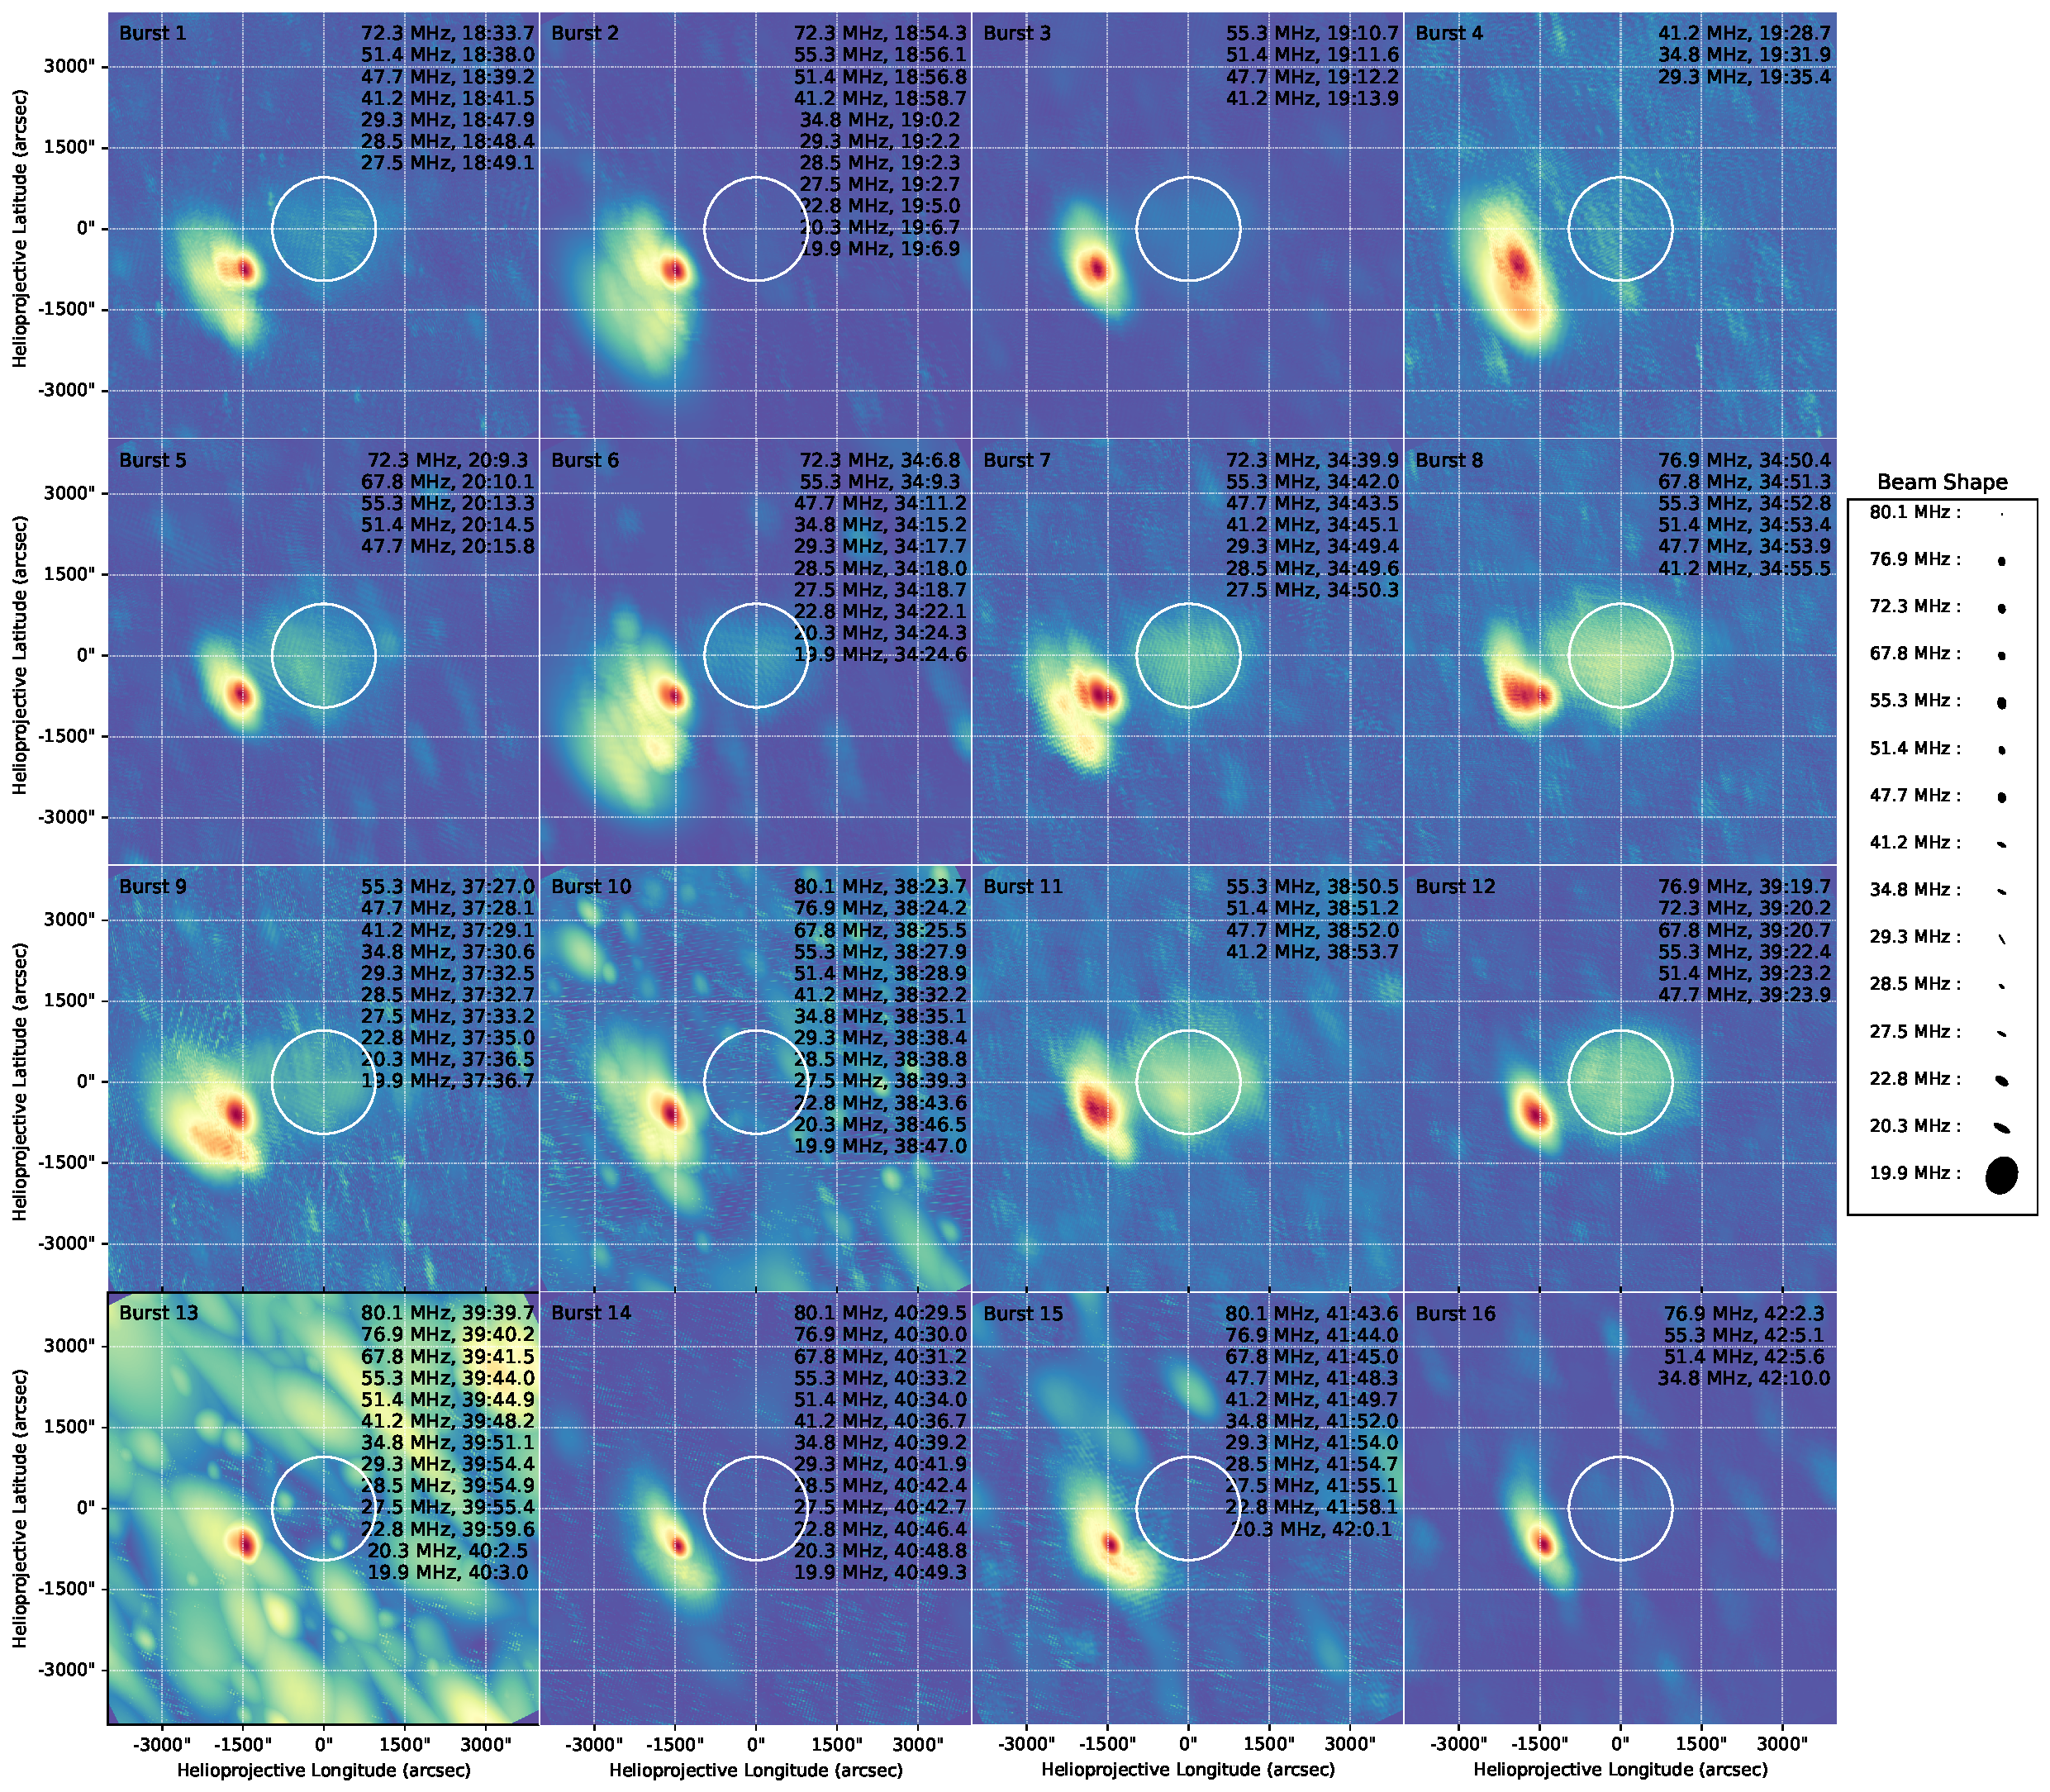
\includegraphics[width=\hsize]{chapter3/figs/subplots.pdf}
\caption{Persistence imaging for the 16 type III bursts detected in the LOFAR dynamic spectrum. The label shows the observation frequencies in MHz and times in (minutes:seconds from 12:00:00 UT). Here, the color coding is not absolute, but rather each panel has its own color code.}
\label{fig_persistence}
\end{figure}

\subsection{Modeling}
To analyze the coronal plasma environment during the events, I utilized standard coronal solutions from MHD simulations by Predictive Science Inc. (PSI) based on the MAS code \citep{mhd_1999}. The PSI MAS coronal solution for April 3, 2019, at 12:00 UT was obtained from the PSI data archive. Initially, I determined the angle between the burst's radial vector and the line of sight (LOS), as well as the complement angle representing the separation between the radial vector and the Earth's perspective. Using the complement angle, I derived the Carrington longitude to extract a longitudinal segment from the MAS datacube, treating it as if it were in the plane of the sky (POS). Longitudinal slices were extracted using the psipy python package. The FORWARD model, responsible for generating synthetic coronal maps, was then applied to the selected data slice. In Figure~\ref{forward2d}, the first radio contour of the sixth type III burst is overlaid on 2D maps of plasma parameters. These parameters include plasma density, temperature, magnetic field strength, plasma beta parameter, total plasma pressure, and Alfven speed. Estimates of local plasma conditions at the centroids' coordinates of type III sources for each frequency band are illustrated in Figure~\ref{scatterplot} for the sixth type III burst.

\section{Results and discussion}
\label{sec_ch3_results}
\subsection{Type III Radio Burst Detection and Characterization}
Radio waves arrived at STEREO one minute before reaching Wind (Fig.~\ref{fig_alldyspec}). However, due to the close proximity to the Sun, the difference in arrival times is within the resolution of the observations, making it inconclusive which spacecraft detected the emission first.

The combined dynamic spectrum from LOFAR and PSP (Fig.~\ref{lofar_psp_burst_detect}) showed limitations in detecting type III bursts compared to LOFAR alone, possibly due to frequency drift and dispersion challenges. Nine bursts were captured from the combined spectrum, while 16 were traced in LOFAR alone (Table~\ref{table_bursts}).

\subsection{Imaging of Radio Emission Sources}
Persistence imaging of the 16 type III bursts from LOFAR (Fig.~\ref{fig_persistence}) suggested a common origin in the south-east quadrant of the solar disk, despite the absence of an active region at that precise location.
A 3D projection of radio source contours onto the coronal magnetic field (Fig.~\ref{fig_3figs}) revealed a south-eastward propagation relative to Earth's perspective. The radio sources aligned with closed field lines in the southern hemisphere and open field lines from the southern coronal hole. However, limitations exist due to outdated magnetic data for AR12738.

The potential origins of type III radio emissions include closed-field lines structures, electron beams from open-field active regions, or from corona acceleration due to magnetic field expansion in active regions.
Furthermore, an inverse relationship between imaging quality and solar radio emission brightness was noted, attributed to calibration solution inaccuracies caused by solar emission leakage into calibrator beam side lobes.

\subsection{Plasma Diagnostics and Magnetic Field Analysis}
The alignment of radio sources (Fig.~\ref{fig_3figs}) with a streamer-like structure near the equator indicates elevated plasma beta, reduced coronal temperature, and diminished Alfven speed. However, the coronal plasma density appeared homogeneous with no prominent structures due to model resolution limitations.
Radio sources for all bursts were found in the same quadrant from Earth's perspective, confined between the equatorial sheet and the southern coronal hole and moving along that boundary.

Variability of coronal plasma quantities at radio sources' centroids was observed (Fig.~\ref{scatterplot}), with coronal temperature increasing with radial distance. Additionally, the behavior of coronal magnetic field, plasma total dynamic pressure, and Alfven speed decreased over distance. Plasma beta parameter sharply increased around 40 MHz, suggesting dominance of plasma pressure over magnetic pressure at that distance from the Sun.

\begin{figure}[!htp]
	\centering
	\begin{subfigure}{0.45\linewidth}
		\centering
		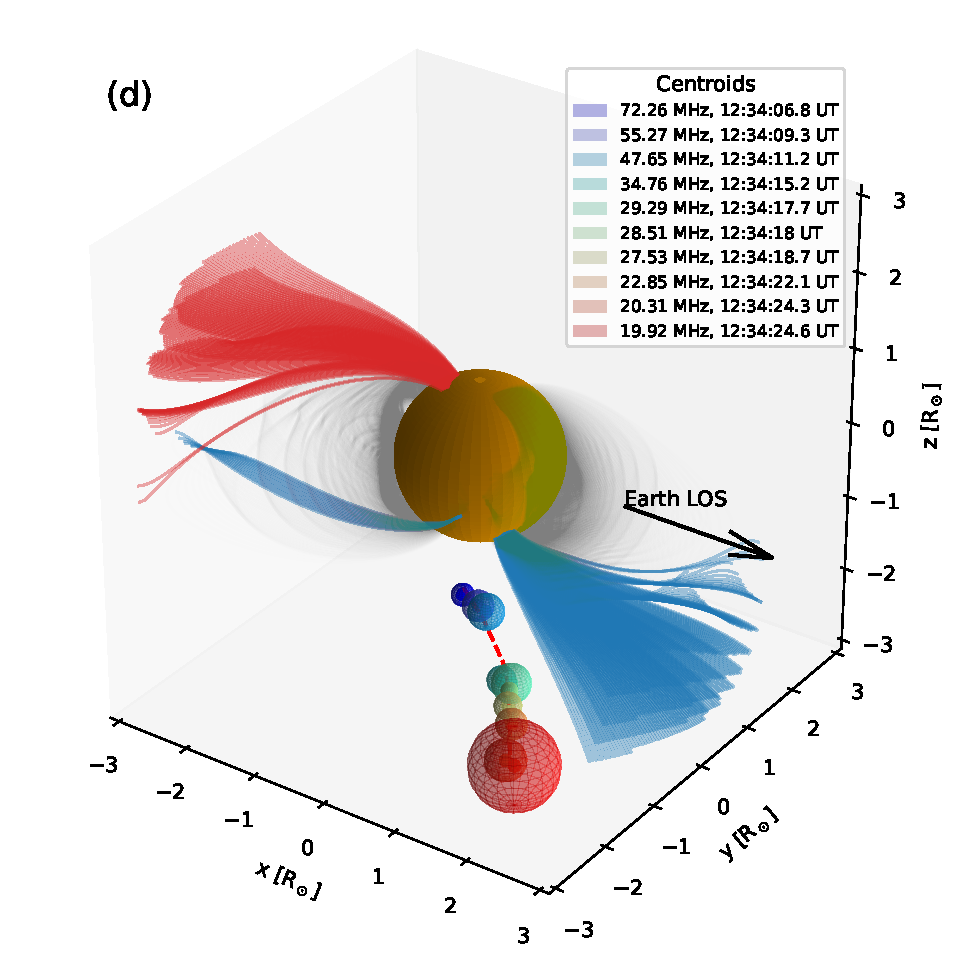
\includegraphics[width=\linewidth]{chapter3/figs/pfss3d_radSources_burst_angle.pdf}
		\label{subfig:a}
	\end{subfigure}
	\hfill
	\begin{subfigure}{0.45\linewidth}
		\centering
		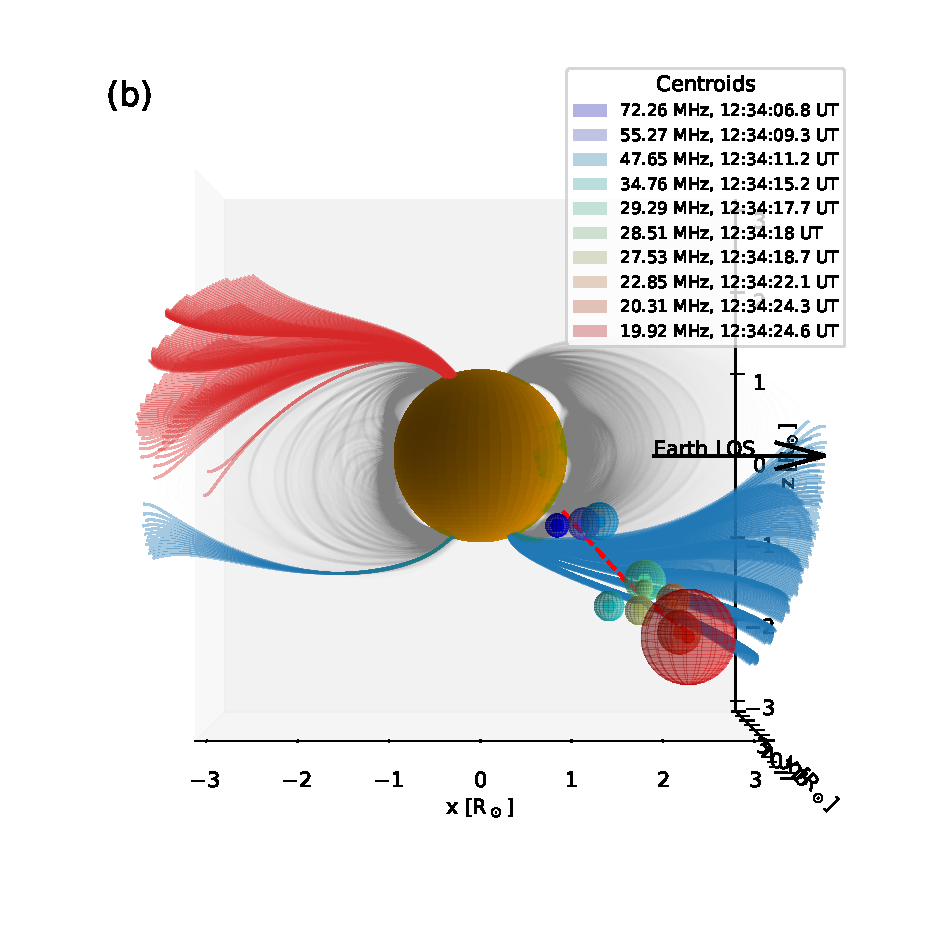
\includegraphics[width=\linewidth]{chapter3/figs/pfss3d_radSources_burst_side.pdf}
		\label{subfig:b}
	\end{subfigure}
	
	\begin{subfigure}{0.45\linewidth}
		\centering
		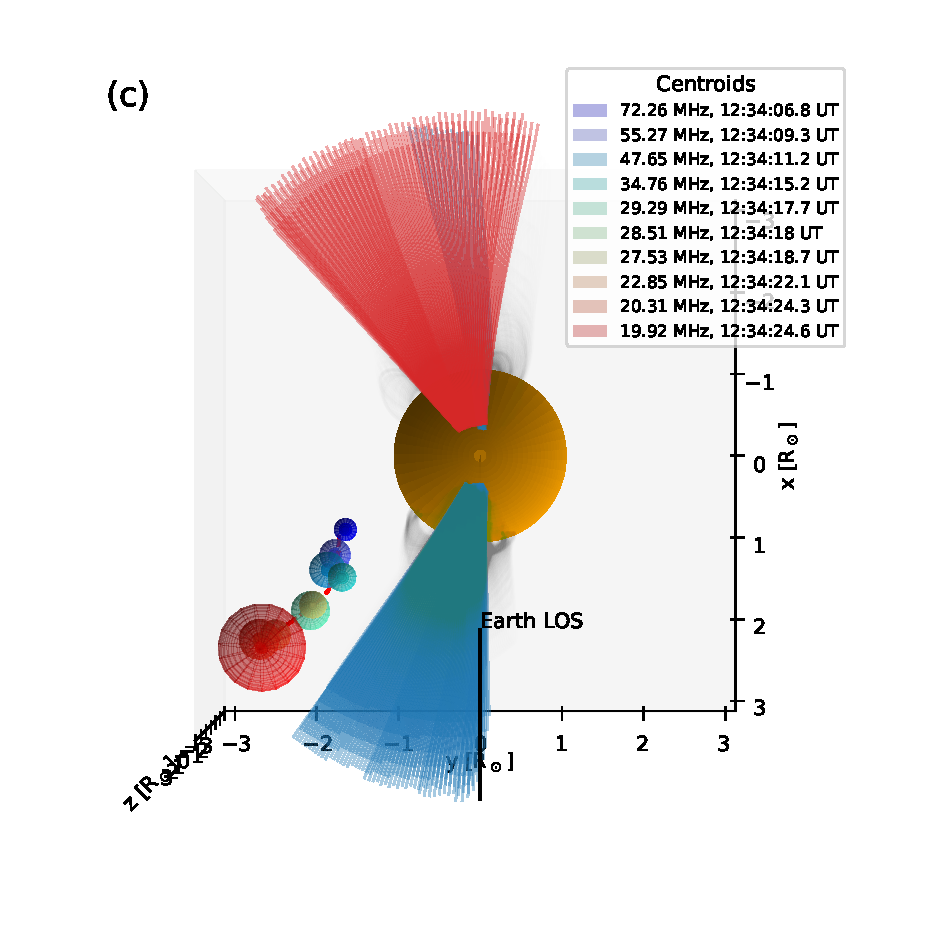
\includegraphics[width=\linewidth]{chapter3/figs/pfss3d_radSources_burst_top.pdf}
		\label{subfig:c}
	\end{subfigure}
	\hfill
	\begin{subfigure}{0.45\linewidth}
		\centering
		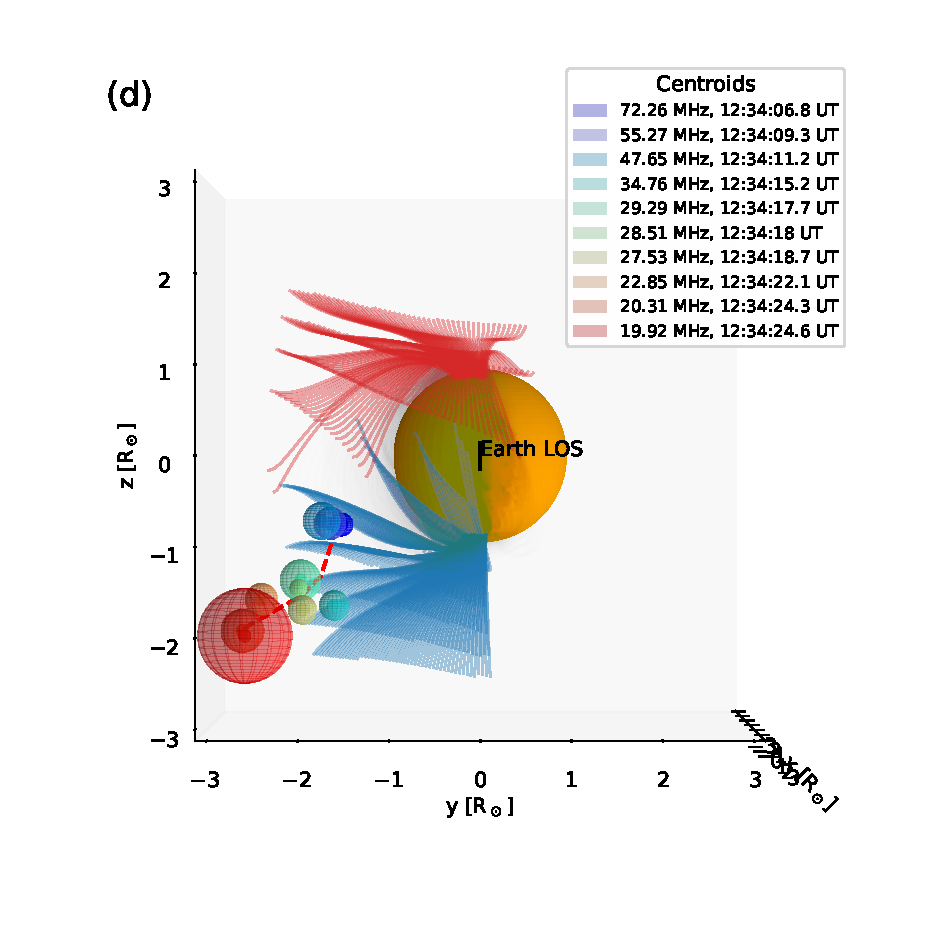
\includegraphics[width=\linewidth]{chapter3/figs/pfss3d_radSources_burst_front.pdf}
		\label{subfig:d}
	\end{subfigure}
	\caption{Different viewing angles for the deprojection of the radio sources of the sixth burst using the 2.5$\times$Newkirk electron-density model on the PFSS solution. The black arrow points toward the Earth's LOS. The $yz$ plane is the POS as seen from the Earth. The red dashed line is a spline curve fit for the sources' centroids. The red, black, and blue curves are the open northern, closed, and open southern field lines, respectively. The opacity of the closed field lines is decreased for better visualization.}
	\label{fig_3figs}
\end{figure}

\begin{figure}[!htp]
	\centering
	\includegraphics[width=0.98\textwidth]{chapter3/figs/LOFAR_FORWARD_plasma_diag_forwtime_2019-04-01T03-42-06.452.pdf}
	\caption{Synthesized maps of plasma parameters obtained using the FORWARD toolset, with the 70\%-contour of radio emission of the sixth burst at the first timestamp (12:34:06.8 UT) at the frequency of 72.26 MHz depicted on top of the 2D POS cuts. The left column represents, from top to bottom, plasma density, magnetic field, and the total plasma dynamic pressure. The right column represents, from top to bottom, the temperature, plasma beta, and the Alfven speed.}
	\label{forward2d}
\end{figure}

\begin{figure}[!htp]
	\centering
	\includegraphics[width=\textwidth]{chapter3/figs/scatterplots_FORWARD_plasma_diagnostics_2019-04-01_4R.pdf}
	\caption{Coronal plasma parameters sampled from the 2D maps by the source centroids. The top panel shows (from left to right) the plasma density profiles from the MAS model, 2.5×Newkirk model, and the theoretical densities under the fundamental and harmonic assumptions, plasma temperature, and magnetic field. The bottom panel shows, from left to right, the total plasma dynamic pressure, Alfven speed, and plasma beta. The x-axis is inverted to demonstrate a progression of increasing radial distance from the Sun as the observer moves towards the right.}
	\label{scatterplot}
\end{figure}

Comparison of density profiles (Fig.~\ref{scatterplot}) indicated significant differences between MAS and FORWARD modeling results compared to the 2.5$\times$Newkirk density model and theoretical expectations. The discrepancy, even after accounting for enhancement factors, suggests possible scattering effects or stealth CMEs affecting density observations, highlighting limitations in current modeling and suggesting the need for additional physics to characterize density distribution accurately.

\section{Summary and conclusions}
\label{sec_ch3_conclusions}
In this study \citep{mnedal_2023b}, a series of 16 type III bursts observed on April 3, 2019, during the PSP's near-Sun encounter, were analyzed using PSP/FIELDS and LOFAR. These bursts, spanning nearly 20 minutes, occurred amidst relative solar quietness with a dominant active region on the solar disk. A semi-automated pipeline aligned PSP and LOFAR observations, facilitating analysis of burst characteristics like frequency drift and electron beam speeds, suggesting their interrelation.

Interferometric imaging revealed a single source for these bursts in the solar corona's southeast limb. Various potential origins for the bursts were discussed, including impulsive events \citep{ishikawa_2017, che_2018, chhabra_2021}, plasma upflows \citep{harra_2021}, and magnetic reconnection \citep{gopalswamy_2022}. Magnetic extrapolation indicated no open potential field lines to active regions AR12737 or AR12738, consistent with prior findings.

Integration of burst source location with magnetic modeling suggested discrepancies, possibly due to scattering effects. Scattering and propagation effects were found significant, impacting burst location determination. Future investigations, including the TDoA technique and Solar Orbiter observations, were proposed.

The study highlighted LOFAR's efficacy in characterizing solar eruptive events and quiet periods, with implications for space weather monitoring. Future work aims to automate burst analysis and investigate their relation to solar surface activity.
Additionally, analysis using LOFAR imaging and MAS modeling indicated discrepancies between observed and modeled burst trajectories, emphasizing the need for model refinements.

Overall, this study underscores the importance of considering scattering effects and refining models to enhance understanding of solar radio emissions' propagation in the corona \citep{kontar_2019, kontar_2023, chen_2023}.